%%%%%%%%%%%%%%%%%%%%%%%%%%%%%%%%%%%%%%%%%%%%%%%%%%%%%%%%%%%%%%%%%%%%%%%%%%%%%%%%
% CSC2059 Practical 9
%%%%%%%%%%%%%%%%%%%%%%%%%%%%%%%%%%%%%%%%%%%%%%%%%%%%%%%%%%%%%%%%%%%%%%%%%%%%%%%%

\documentclass{csc2059practical}

% Additional packages used by this practical.
% TikZ will be used during the visual design pass.
\usepackage{tikz}
\usetikzlibrary{arrows.meta, positioning, fit, backgrounds}
\usepackage{fontawesome5}
\usepackage{booktabs}


\setpracticalnumber{9}

\setpracticaltitle{Beyond the trees}

\setpracticalsubtitle{Modelling relationships with Graphs}

\setpracticalauthor{
Dr Giuseppe Trombino\\
School of Electronics, Electrical Engineering and Computer Science\\
Queen's University Belfast
}
\setpracticaldate{}

\usetikzlibrary{arrows.meta,positioning,calc}

% Shared TikZ styles for graph figures

\tikzset{
    airport/.style={
        circle,
        draw=black!70,
        fill=white,
        line width=0.9pt,
        minimum size=10mm,
        inner sep=1pt,
        font=\ttfamily\small\bfseries
    },
    route/.style={
        draw=black!45,
        line width=0.8pt,
        line cap=round
    },
    route faded/.style={
        draw=black!18,
        line width=0.8pt,
        line cap=round
    },
    route highlighted/.style={
        draw=blue!70!black,
        line width=1.8pt,
        line cap=round
    },
    airport visited/.style={
        airport,
        fill=blue!12,
        draw=blue!65!black
    },
    airport active/.style={
        airport,
        fill=blue!30,
        draw=blue!80!black,
        line width=1.2pt
    },
    component main/.style={
        airport,
        fill=green!15,
        draw=green!45!black
    },
    component secondary/.style={
        airport,
        fill=orange!18,
        draw=orange!60!black
    },
    component isolated/.style={
        airport,
        fill=black!7,
        draw=black!45
    },
    route weight/.style={
        midway,
        fill=white,
        inner sep=1.5pt,
        font=\scriptsize\sffamily
    },
    adjacency airport/.style={
        rectangle,
        rounded corners=2pt,
        draw=black!70,
        fill=white,
        minimum width=12mm,
        minimum height=7mm,
        font=\ttfamily\small\bfseries
    },
    adjacency neighbour/.style={
        rectangle,
        rounded corners=2pt,
        draw=black!45,
        fill=black!4,
        minimum width=12mm,
        minimum height=7mm,
        font=\ttfamily\small
    },
    adjacency arrow/.style={
        ->,
        >=stealth,
        draw=black!45,
        line width=0.7pt
    },
    adjacency empty/.style={
        font=\sffamily\small\itshape,
        text=black!55
    },
    order badge/.style={
        circle,
        draw=blue!70!black,
        fill=white,
        minimum size=5mm,
        inner sep=0pt,
        font=\sffamily\scriptsize\bfseries,
        text=blue!70!black
    },
    stack frame/.style={
        rectangle,
        rounded corners=2pt,
        draw=black!45,
        fill=white,
        minimum width=31mm,
        minimum height=7mm,
        align=center,
        font=\ttfamily\scriptsize
    },
    stack frame active/.style={
        stack frame,
        draw=blue!75!black,
        fill=blue!18,
        line width=1.1pt
    },
    stack arrow/.style={
        ->,
        >=stealth,
        draw=black!45,
        line width=0.7pt
    },
    figure annotation/.style={
        font=\sffamily\small,
        text=black!65,
        align=center
    },
    cycle highlighted/.style={
        draw=red!70!black,
        line width=1.8pt,
        line cap=round
    },
    cycle direction/.style={
        ->,
        >=stealth,
        draw=red!70!black,
        line width=1.8pt,
        line cap=round
    },
    cycle airport/.style={
        airport,
        fill=red!12,
        draw=red!65!black,
        line width=1.2pt
    },
    cycle annotation/.style={
        rectangle,
        rounded corners=2pt,
        draw=red!55!black,
        fill=red!5,
        inner sep=5pt,
        align=left,
        text width=42mm,
        font=\sffamily\small
    },
    visited annotation/.style={
        cycle annotation,
        draw=green!45!black,
        fill=green!6
    },
    component main route/.style={
    draw=green!45!black,
    line width=1.1pt,
    line cap=round
    },
    component secondary route/.style={
        draw=orange!60!black,
        line width=1.1pt,
        line cap=round
    },
    component isolated label/.style={
        font=\sffamily\scriptsize\itshape,
        text=black!55,
        align=center
    },
    weighted route/.style={
    draw=purple!55!black,
    line width=1.1pt,
    line cap=round
    },
    route weight/.style={
        midway,
        fill=white,
        draw=purple!30!black,
        rounded corners=1pt,
        inner xsep=3pt,
        inner ysep=1.5pt,
        font=\sffamily\scriptsize\bfseries,
        text=purple!65!black
    },
    weighted airport/.style={
        airport,
        fill=purple!8,
        draw=purple!55!black
    },
    weight annotation/.style={
        rounded corners=2pt,
        draw=purple!35!black,
        fill=purple!5,
        inner sep=5pt,
        align=left,
        text width=43mm,
        font=\sffamily\small
    },
}
% Reusable airport network layout and drawing commands.

\newcommand{\AirportNetworkCoordinates}{%
    % Main connected component
    \coordinate (BFS) at (2.4, -0.5);
    \coordinate (LHR) at (6.9, -1.4);
    \coordinate (AMS) at (5.0,  0.8);
    \coordinate (CDG) at (7.6,  1.8);
    
    \coordinate (FRA) at (4.0,  3.2);
    \coordinate (FCO) at (0.2,  0.8);
    \coordinate (MAD) at (4.4, -2.5);
    \coordinate (LIS) at (0.2, -2.5);

    % Secondary connected component
    \coordinate (KEF) at (0.2, 3.1);
    \coordinate (OSL) at (2.5, 3.4);

    % Isolated airports
    \coordinate (EDI) at (8.8, 0.8);
    \coordinate (ATH) at (8.8, -2.2);
}
\newcommand{\DrawAirportVertices}{%
    \node[airport] at (BFS) {BFS};
    \node[airport] at (LHR) {LHR};
    \node[airport] at (AMS) {AMS};
    \node[airport] at (CDG) {CDG};
    \node[airport] at (FRA) {FRA};
    \node[airport] at (FCO) {FCO};
    \node[airport] at (MAD) {MAD};
    \node[airport] at (LIS) {LIS};

    \node[airport] at (KEF) {KEF};
    \node[airport] at (OSL) {OSL};

    \node[airport] at (EDI) {EDI};
    \node[airport] at (ATH) {ATH};
}

\newcommand{\DrawAirportRoutes}[1][route]{%
    % Main connected component
    \draw[#1] (BFS) -- (LHR);
    \draw[#1] (BFS) -- (AMS);
    \draw[#1] (BFS) -- (FCO);

    \draw[#1] (LHR) -- (CDG);
    \draw[#1] (LHR) -- (MAD);

    \draw[#1] (AMS) -- (CDG);
    \draw[#1] (AMS) -- (FRA);

    \draw[#1] (CDG) -- (FRA);

    \draw[#1] (FRA) -- (FCO);

    \draw[#1] (FCO) -- (LIS);

    \draw[#1] (MAD) -- (LIS);

    % Secondary connected component
    \draw[#1] (KEF) -- (OSL);
}
\newcommand{\DrawAdjacencyList}{%
    % BFS
    \node[adjacency airport] (bfs) at (0,0) {BFS};
    \node[adjacency neighbour] (bfs-lhr) at (2,0) {LHR};
    \node[adjacency neighbour] (bfs-ams) at (4,0) {AMS};
    \node[adjacency neighbour] (bfs-fco) at (6,0) {FCO};

    \draw[adjacency arrow] (bfs) -- (bfs-lhr);
    \draw[adjacency arrow] (bfs-lhr) -- (bfs-ams);
    \draw[adjacency arrow] (bfs-ams) -- (bfs-fco);

    % LHR
    \node[adjacency airport] (lhr) at (0,-1) {LHR};
    \node[adjacency neighbour] (lhr-bfs) at (2,-1) {BFS};
    \node[adjacency neighbour] (lhr-cdg) at (4,-1) {CDG};
    \node[adjacency neighbour] (lhr-mad) at (6,-1) {MAD};

    \draw[adjacency arrow] (lhr) -- (lhr-bfs);
    \draw[adjacency arrow] (lhr-bfs) -- (lhr-cdg);
    \draw[adjacency arrow] (lhr-cdg) -- (lhr-mad);

    % EDI
    \node[adjacency airport] (edi) at (0,-2) {EDI};
    \node[adjacency empty, anchor=west] at (1.4,-2) {no routes};
}

\newcommand{\DrawDFSActivePath}{%
    \draw[route highlighted] (BFS) -- (LHR);
    \draw[route highlighted] (LHR) -- (CDG);
    \draw[route highlighted] (CDG) -- (AMS);
}

\newcommand{\DrawDFSProgressVertices}{%
    % Previously visited airports
    \node[
        airport visited,
        label={[order badge]135:1}
    ] at (BFS) {BFS};

    \node[
        airport visited,
        label={[order badge]-45:2}
    ] at (LHR) {LHR};

    \node[
        airport visited,
        label={[order badge]45:3}
    ] at (CDG) {CDG};

    % Current recursive call
    \node[
        airport active,
        label={[order badge]135:4}
    ] at (AMS) {AMS};

    % Airports not yet visited
    \node[airport] at (FRA) {FRA};
    \node[airport] at (FCO) {FCO};
    \node[airport] at (MAD) {MAD};
    \node[airport] at (LIS) {LIS};

    % Other connected component
    \node[airport] at (KEF) {KEF};
    \node[airport] at (OSL) {OSL};

    % Isolated airports
    \node[airport] at (EDI) {EDI};
    \node[airport] at (ATH) {ATH};
}

\newcommand{\DrawDFSCallStack}{%
    \node[
        figure annotation,
        font=\sffamily\small\bfseries
    ] at (0,0.6) {Active recursive calls};

    \node[stack frame] (call-bfs) at (0,0) {
        depthFirst(BFS)
    };

    \node[stack frame] (call-lhr) at (0,-1.0) {
        depthFirst(LHR)
    };

    \node[stack frame] (call-cdg) at (0,-2.0) {
        depthFirst(CDG)
    };

    \node[stack frame active] (call-ams) at (0,-3.0) {
        depthFirst(AMS)
    };

    \draw[stack arrow] (call-bfs) -- (call-lhr);
    \draw[stack arrow] (call-lhr) -- (call-cdg);
    \draw[stack arrow] (call-cdg) -- (call-ams);

    \node[
        figure annotation,
        anchor=west,
        text=blue!70!black
    ] at (0,-3.5) {current call};
}

\newcommand{\HighlightAirportCycle}{%
    \draw[cycle direction] (BFS) -- (LHR);
    \draw[cycle direction] (LHR) -- (CDG);
    \draw[cycle direction] (CDG) -- (AMS);
    \draw[cycle direction] (AMS) -- (BFS);
}

\newcommand{\DrawCycleVertices}{%
    % Airports forming the cycle
    \node[airport active] at (BFS) {BFS};
    \node[airport active] at (LHR) {LHR};
    \node[airport active] at (CDG) {CDG};
    \node[airport active] at (AMS) {AMS};

    % Remaining airports
    \node[airport] at (FRA) {FRA};
    \node[airport] at (FCO) {FCO};
    \node[airport] at (MAD) {MAD};
    \node[airport] at (LIS) {LIS};

    \node[airport] at (KEF) {KEF};
    \node[airport] at (OSL) {OSL};

    \node[airport] at (EDI) {EDI};
    \node[airport] at (ATH) {ATH};
}

\newcommand{\DrawVisitedExplanation}{%
    \node[cycle annotation] at (0,0) {
        \textbf{Without \texttt{visited[]}:}

        \medskip

        \texttt{BFS}
        $\rightarrow$
        \texttt{LHR}
        $\rightarrow$
        \texttt{CDG}
        $\rightarrow$
        \texttt{AMS}
        $\rightarrow$
        \texttt{BFS}
        $\rightarrow \cdots$

        \medskip

        The traversal can repeatedly return to airports that it has already explored.
    };

    \node[
        cycle annotation,
        draw=green!45!black,
        fill=green!6,
        text width=42mm
    ] at (0,-3.2) {
        \textbf{With \texttt{visited[]}:}

        \medskip

        Before following a route, DFS checks whether the destination has already been visited.

        \medskip

        Each airport is therefore processed at most once.
    };
}

\newcommand{\DrawConnectedComponentRoutes}{%
    % Main connected component
    \draw[component main route] (BFS) -- (LHR);
    \draw[component main route] (BFS) -- (AMS);
    \draw[component main route] (BFS) -- (FCO);

    % Retain the remaining routes from the main component here,
    % using component main route.
    \draw[component main route] (LHR) -- (CDG);
    \draw[component main route] (LHR) -- (MAD);

    \draw[component main route] (AMS) -- (CDG);
    \draw[component main route] (AMS) -- (FRA);

    \draw[component main route] (CDG) -- (FRA);

    \draw[component main route] (FRA) -- (FCO);

    \draw[component main route] (FCO) -- (LIS);

    \draw[component main route] (MAD) -- (LIS);


    % Secondary connected component
    \draw[component secondary route] (KEF) -- (OSL);
}

\newcommand{\DrawConnectedComponentVertices}{%
    % Main connected component
    \node[component main] at (BFS) {BFS};
    \node[component main] at (LHR) {LHR};
    \node[component main] at (AMS) {AMS};
    \node[component main] at (CDG) {CDG};
    \node[component main] at (FRA) {FRA};
    \node[component main] at (FCO) {FCO};
    \node[component main] at (MAD) {MAD};
    \node[component main] at (LIS) {LIS};

    % Secondary connected component
    \node[component secondary] at (KEF) {KEF};
    \node[component secondary] at (OSL) {OSL};

    % Isolated components
    \node[component isolated] at (EDI) {EDI};
    \node[component isolated] at (ATH) {ATH};
}

\newcommand{\DrawConnectedComponentLabels}{%
    \node[
        figure annotation,
        text=green!45!black,
        font=\sffamily\small\bfseries
    ] at (4.6,-3.45) {Main connected component};

    \node[
        figure annotation,
        text=orange!65!black,
        font=\sffamily\small\bfseries
    ] at (1.35,4.05) {Secondary component};

    \node[
        component isolated label
    ] at (8.8,-3.05) {isolated airports};
}

\newcommand{\DrawWeightedAirportNetwork}{%
    \DrawAirportRoutes[weighted route]

    % Illustrative route distances
    \path (BFS) -- (LHR)
        node[route weight, above, sloped] {510 km};

    \path (BFS) -- (AMS)
        node[route weight, above, sloped] {760 km};

    \path (BFS) -- (FCO)
        node[route weight, above, sloped] {1,950 km};

    \path (LHR) -- (CDG)
        node[route weight, above, sloped] {350 km};

    \path (LHR) -- (MAD)
        node[route weight, below, sloped] {1,260 km};

    \path (CDG) -- (AMS)
        node[route weight, above, sloped] {430 km};

    \path (KEF) -- (OSL)
        node[route weight, below, sloped] {1,750 km};
}

\newcommand{\DrawWeightedAirportVertices}{%
    \node[weighted airport] at (BFS) {BFS};
    \node[weighted airport] at (LHR) {LHR};
    \node[weighted airport] at (AMS) {AMS};
    \node[weighted airport] at (CDG) {CDG};
    \node[weighted airport] at (FRA) {FRA};
    \node[weighted airport] at (FCO) {FCO};
    \node[weighted airport] at (MAD) {MAD};
    \node[weighted airport] at (LIS) {LIS};

    \node[weighted airport] at (KEF) {KEF};
    \node[weighted airport] at (OSL) {OSL};

    \node[component isolated] at (EDI) {EDI};
    \node[component isolated] at (ATH) {ATH};
}

\newcommand{\DrawWeightedGraphExplanation}{%
    \node[weight annotation] at (0,0) {
        \textbf{Weighted graph}

        \medskip

        Each route stores an additional value called a
        \emph{weight}.

        \medskip

        A weight might represent:

        \smallskip

        \begin{tabular}{@{}l@{}}
            $\bullet$ distance\\
            $\bullet$ journey time\\
            $\bullet$ ticket cost
        \end{tabular}

        \medskip

        A shortest-path algorithm compares the total weight of
        alternative routes.
    };
}


\begin{document}

\maketitle

\tableofcontents
\clearpage


%%%%%%%%%%%%%%%%%%%%%%%%%%%%%%%%%%%%%%%%%%%%%%%%%%%%%%%%%%%%%%%%%%%%%%%%%%%%%%%%
% Introduction
%%%%%%%%%%%%%%%%%%%%%%%%%%%%%%%%%%%%%%%%%%%%%%%%%%%%%%%%%%%%%%%%%%%%%%%%%%%%%%%%

\frontsection{Introduction}

How would you represent an airline network in a computer?

A list of airports would tell you which airports exist, but it would not tell
you where passengers can travel. To model the network properly, you must also
record the routes that connect those airports.

This distinction leads to one of the most important ideas in computer science:

\begin{quote}
A graph represents a collection of objects together with the relationships
between them.
\end{quote}

The objects in a graph are called \textbf{vertices}. In this practical, each
vertex represents an airport. The relationships between vertices are called
\textbf{edges}. Each edge in the airport network represents a direct flight
route between two airports.

Graphs can model many different kinds of connected information. For example:

\begin{itemize}
\item people connected through friendships in a social network;
\item locations connected by roads or railway lines;
\item computers connected through a communication network;
\item web pages connected through hyperlinks;
\item airports connected through flight routes.
\end{itemize}

Although these applications appear very different, their underlying structure
is the same: a collection of entities and a collection of relationships between
them.

In earlier practicals, you worked with linear data structures such as arrays and
linked lists, where elements follow a clear sequence. You also explored trees,
where nodes form a hierarchy and each node has a well-defined position beneath
a root.

Graphs remove many of those restrictions. A vertex may be connected to several
other vertices, multiple paths may lead to the same destination, and cycles may
allow a traversal to return to a vertex that has already been encountered.
Graphs can also contain separate groups of vertices that are not connected to
one another.

These properties make graphs powerful, but they also introduce new design
questions:

\begin{itemize}
\item How should vertices and edges be represented?
\item How can a program explore the network without repeatedly visiting the
same vertices?
\item How can we determine which parts of a network are connected?
\end{itemize}

In this practical, you will answer these questions by constructing an undirected
airport network and implementing a recursive \textbf{Depth-First Search (DFS)}
algorithm.

You will begin by adding the two fundamental parts of a graph separately:

\begin{enumerate}
\item the airports that form its vertices;
\item the flight routes that form its edges.
\end{enumerate}

You will then use a supplied dataset loader to construct a larger network,
implement DFS to explore the airports reachable from a chosen starting point,
and investigate how adding or removing routes changes the connectivity of the
network.

Public Catch2 tests will guide the implementation of each new behaviour. The
final part of the practical will move beyond simply making those tests pass:
you will predict how changes affect the graph, test those predictions, and
explain the results.

\begin{engineeringquestion}
How can we represent and explore a network in which each object may be connected
to several others?
\end{engineeringquestion}

\begin{importantnote}
A graph is not simply a more complicated tree.

A tree is a particular kind of graph with a restricted structure. General
graphs may contain cycles, alternative paths, isolated vertices and separate
connected components. These possibilities affect both how a graph is stored and
how it must be traversed.
\end{importantnote}

%%%%%%%%%%%%%%%%%%%%%%%%%%%%%%%%%%%%%%%%%%%%%%%%%%%%%%%%%%%%%%%%%%%%%%%%%%%%%%%%
% Learning Outcomes
%%%%%%%%%%%%%%%%%%%%%%%%%%%%%%%%%%%%%%%%%%%%%%%%%%%%%%%%%%%%%%%%%%%%%%%%%%%%%%%%

\begin{learningoutcomes}

By the end of this practical, you should be able to:

\begin{itemize}
\item explain how vertices and edges represent objects and relationships in
a graph;
\item distinguish an undirected graph from the hierarchical tree structures
explored previously;
\item construct an undirected graph by adding vertices and edges while
preserving the rules of the data structure;
\item explain how an adjacency-list representation records the neighbours
of each vertex;
\item implement a recursive Depth-First Search algorithm that safely
traverses a graph containing cycles;
\item use a visited structure to prevent vertices from being processed more
than once;
\item use DFS results to identify and reason about connected components;
\item predict, test and explain how adding or removing edges changes the
connectivity of a graph.
\end{itemize}

\end{learningoutcomes}

%%%%%%%%%%%%%%%%%%%%%%%%%%%%%%%%%%%%%%%%%%%%%%%%%%%%%%%%%%%%%%%%%%%%%%%%%%%%%%%%
% Before You Begin
%%%%%%%%%%%%%%%%%%%%%%%%%%%%%%%%%%%%%%%%%%%%%%%%%%%%%%%%%%%%%%%%%%%%%%%%%%%%%%%%

\frontsection{Before You Begin}

This practical introduces a new data structure, but it builds on programming
skills and algorithmic ideas developed throughout the module.

Before beginning, check that you can recognise and use the following:

\begin{itemize}
\item compiling and running C++ programs using Visual Studio Code and a
Makefile;
\item running public Catch2 tests and interpreting a failed assertion;
\item using a failing test to identify the next small behaviour to
implement;
\item separating declarations in header files from implementations in
source files;
\item reading and modifying a C++ class implementation;
\item storing objects in a fixed-size array and using a counter to record
how many positions are occupied;
\item using loops to search arrays and process their occupied elements;
\item passing arrays to functions;
\item recognising a recursive function, its stopping condition and its
recursive call;
\item tracing the order in which recursive calls are made.
\end{itemize}

The practical builds particularly closely on the recursive reasoning developed
in Practical 7. There, recursion followed the child relationships of a tree. In
this practical, the recursive algorithm will follow the neighbouring vertices
of a graph.

The central pattern remains familiar:

\begin{quote}
Process the current object, then apply the same operation to the objects
connected to it.
\end{quote}

However, graphs introduce one important complication. In a tree, following child
relationships eventually reaches a leaf. In a graph, routes may form cycles and
lead back to an airport that has already been visited.

For example, a network might contain the routes:

\begin{center}
\mintinline{text}{BFS – LHR – CDG – BFS}
\end{center}

Without recording which airports have already been processed, a recursive
traversal could continue around this cycle indefinitely.

You will address this problem in Part C using a Boolean array that records the
visited state of every airport.

\begin{importantnote}
You do not need any previous experience of graph theory before starting this
practical.

The opening section will introduce the graph terminology and representation
needed for the coding activities. Your existing understanding of arrays,
classes, tests and recursion provides the programming foundation.
\end{importantnote}

\begin{tipbox}
If recursive calls still feel unfamiliar, briefly revisit the tracing
activities from Practical 7.

Focus on three questions:

\begin{enumerate}
\item What is being processed by the current call?
\item Which connected object will be passed to the next call?
\item What condition prevents further recursive calls?
\end{enumerate}

In this practical, a fourth question will become equally important:

\begin{quote}
Has this vertex already been visited?
\end{quote}
\end{tipbox}

%%%%%%%%%%%%%%%%%%%%%%%%%%%%%%%%%%%%%%%%%%%%%%%%%%%%%%%%%%%%%%%%%%%%%%%%%%%%%%%%
% Understanding Graphs
%%%%%%%%%%%%%%%%%%%%%%%%%%%%%%%%%%%%%%%%%%%%%%%%%%%%%%%%%%%%%%%%%%%%%%%%%%%%%%%%

\frontsection{Understanding Graphs}

Before writing any code, it is worth taking a few minutes to understand the data
structure you are about to build.

Many of the data structures explored in this module organise data into a
particular shape. Arrays arrange elements in a sequence. Linked lists connect
each element to the next. Trees organise nodes into a hierarchy beneath a single
root.

Graphs take a different approach.

Instead of imposing a particular structure, a graph simply records:

\begin{enumerate}
\item the objects we want to represent;
\item the relationships between those objects.
\end{enumerate}

The objects are called \textbf{vertices} and the relationships between them are
called \textbf{edges}.

In this practical, each airport is represented by a vertex, while each direct
flight route is represented by an edge connecting two airports.

%%%%%%%%%%%%%%%%%%%%%%%%%%%%%%%%%%%%%%%%%%%%%%%%%%%%%%%%%%%%%%%%%%%%%%%%%%%%%%%%

\subsection*{Vertices}

A vertex represents one object within the graph.

For our airport network, every airport is stored as a separate vertex.

Initially, these airports are completely independent.

\begin{figure}[htbp]
    \centering

    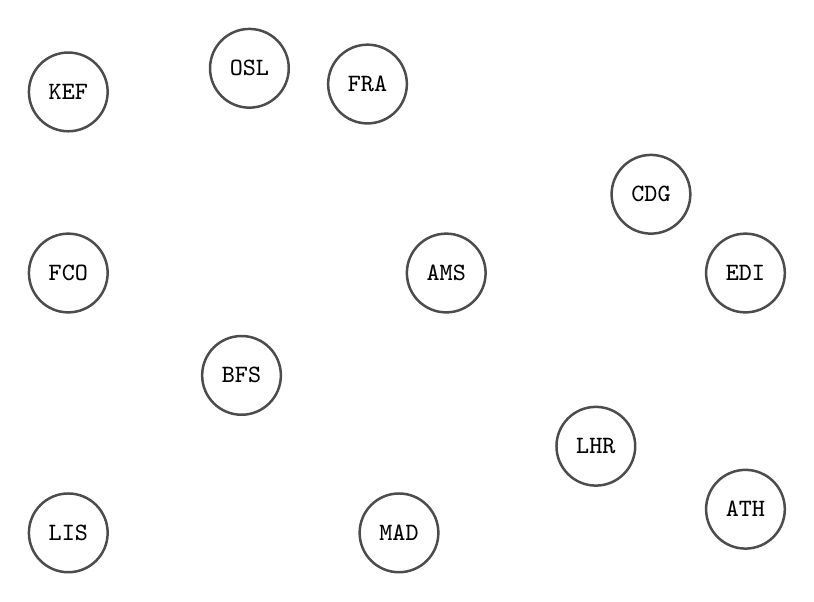
\begin{tikzpicture}
        \AirportNetworkCoordinates
        \DrawAirportVertices
    \end{tikzpicture}

    \caption{Airports represented as vertices in a graph.}
    \label{fig:airport-vertices}
\end{figure}



At this stage, the graph tells us which airports exist, but it provides no
information about where passengers can travel.

%%%%%%%%%%%%%%%%%%%%%%%%%%%%%%%%%%%%%%%%%%%%%%%%%%%%%%%%%%%%%%%%%%%%%%%%%%%%%%%%

\subsection*{Edges}

To describe the network, we must also record the routes that connect airports.

Each route becomes an \textbf{edge} joining two vertices.

\begin{figure}[htbp]
    \centering

    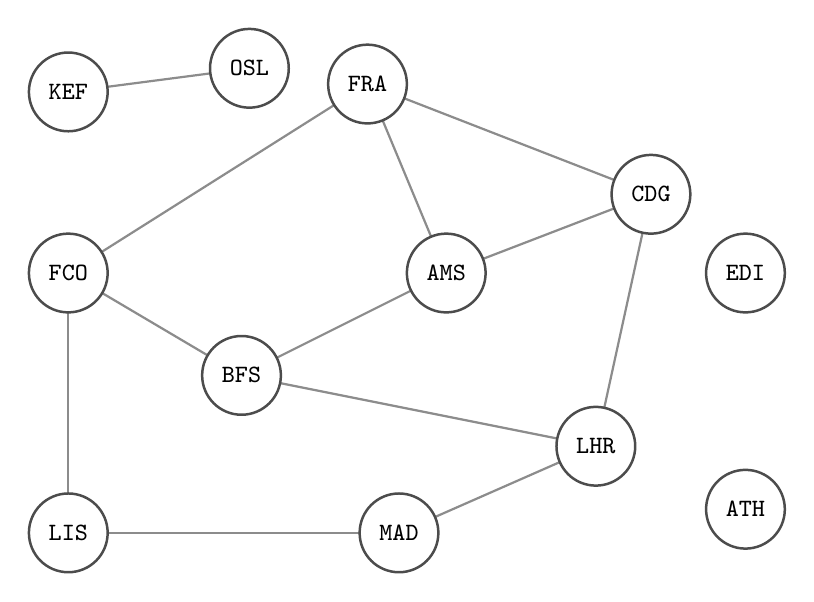
\begin{tikzpicture}
        \AirportNetworkCoordinates
        \DrawAirportRoutes
        \DrawAirportVertices
    \end{tikzpicture}

    \caption{Airports connected by direct flight routes.}
    \label{fig:airport-network}
\end{figure}

Notice that the airports themselves have not changed. We have simply added
relationships between them.

This idea appears in many real-world systems.
\clearpage
For example:

\begin{itemize}
\item in a social network, the vertices are people and the edges represent
friendships;
\item in a road map, the vertices are towns and the edges represent roads;
\item in a computer network, the vertices are devices and the edges
represent communication links.
\end{itemize}

The same graph structure can therefore model many different kinds of problems.

%%%%%%%%%%%%%%%%%%%%%%%%%%%%%%%%%%%%%%%%%%%%%%%%%%%%%%%%%%%%%%%%%%%%%%%%%%%%%%%%

\subsection*{Undirected Graphs}

Some relationships have a direction.

For example, a web page may contain a hyperlink to another page without that
second page linking back.

Other relationships naturally work in both directions.

In this practical, every flight route can be travelled in either direction.
Although the route is entered only once by the user, it will be stored for both
airports.

This makes our airport network an \textbf{undirected graph}.

Whenever a route is added between two airports, both airports will record that
connection.


%%%%%%%%%%%%%%%%%%%%%%%%%%%%%%%%%%%%%%%%%%%%%%%%%%%%%%%%%%%%%%%%%%%%%%%%%%%%%%%%

\subsection*{Building the Airport Network}

Part A of this practical mirrors the way we have introduced graphs in this
section.

You will first add the airports that form the graph’s vertices.

Once those vertices exist, you will connect them by adding flight routes that
form the graph’s edges.

By constructing the graph one step at a time, you will gain a clear
understanding of how its structure develops before moving on to graph traversal
in Part C.

%%%%%%%%%%%%%%%%%%%%%%%%%%%%%%%%%%%%%%%%%%%%%%%%%%%%%%%%%%%%%%%%%%%%%%%%%%%%%%%%
% Getting to Know the Repository
%%%%%%%%%%%%%%%%%%%%%%%%%%%%%%%%%%%%%%%%%%%%%%%%%%%%%%%%%%%%%%%%%%%%%%%%%%%%%%%%

\frontsection{Getting to Know the Repository}

Before implementing any new functionality, it is worth taking a few minutes to
become familiar with the project structure.

As with previous practicals, most of the repository has already been completed
for you. Your task is not to build the entire application from scratch, but to
extend an existing code base by implementing a small number of carefully chosen
functions.

The repository contains examples, public tests and supporting code that work
together to guide your implementation. Rather than trying to understand every
file immediately, begin by identifying the files that are directly relevant to
the first exercise.

%%%%%%%%%%%%%%%%%%%%%%%%%%%%%%%%%%%%%%%%%%%%%%%%%%%%%%%%%%%%%%%%%%%%%%%%%%%%%%%%

\subsection*{Repository Structure}

The repository is organised into several folders, each with a specific purpose.

\begin{center}
\begin{tabular}{p{0.34\textwidth} p{0.58\textwidth}}
\toprule
\textbf{Path} & \textbf{Purpose} \\
\midrule
\texttt{include/} & Header files defining the graph classes. \\
\texttt{src/}     & Source files containing the implementations. \\
\texttt{data/}    & Example datasets used later in the practical. \\
\texttt{examples/}& Demonstration programs. \\
\texttt{tests/}   & Public Catch2 tests. \\
\bottomrule
\end{tabular}
\end{center}


For Part A, you will spend almost all of your time working with the files in the
\texttt{include/} and \texttt{src/} directories.

%%%%%%%%%%%%%%%%%%%%%%%%%%%%%%%%%%%%%%%%%%%%%%%%%%%%%%%%%%%%%%%%%%%%%%%%%%%%%%%%

\subsection*{The Core Graph Classes}

Three classes work together to represent the airport network.

Each class has a different responsibility.

\begin{description}
\item[\texttt{FlightRoute}] Represents a single flight route from one
airport to another. Each route stores the destination airport together with
information about the connection.

\item[\texttt{Airport}] Represents a single airport. Each airport stores its
identifying information together with the flight routes that leave that
airport.
\item[\texttt{Graph}] Represents the complete airport network. It stores all
airports and provides the operations used to build and explore the graph.

\end{description}

Separating these responsibilities makes the code easier to understand and
maintain. Each class has a clear purpose within the overall design.

%%%%%%%%%%%%%%%%%%%%%%%%%%%%%%%%%%%%%%%%%%%%%%%%%%%%%%%%%%%%%%%%%%%%%%%%%%%%%%%%

\subsection*{What Has Already Been Implemented?}

As in previous practicals, much of the supporting code has already been provided
for you.

For example, the repository already contains:

\begin{itemize}
\item constructors and helper functions;
\item example programs demonstrating the graph;
\item dataset loading utilities used later in the practical;
\item public Catch2 tests for each exercise.
\end{itemize}

This allows you to concentrate on the algorithms rather than spending time
writing infrastructure.

%%%%%%%%%%%%%%%%%%%%%%%%%%%%%%%%%%%%%%%%%%%%%%%%%%%%%%%%%%%%%%%%%%%%%%%%%%%%%%%%

\subsection*{Your First Tasks}

In Part A, you will implement the two operations needed to build the graph.

The implementation deliberately follows the way graphs were introduced earlier
in this practical.

\begin{enumerate}
\item Implement \mintinline{cpp}{addAirport()} to add vertices to the graph.
\item Implement \mintinline{cpp}{addRoute()} to connect those vertices with
edges.
\end{enumerate}

After each function is implemented, run the public tests before moving on to the
next task.

Building the graph one small step at a time will make it much easier to
understand how the data structure grows as new airports and routes are added.

\begin{tipbox}
Do not try to understand every function in \texttt{Graph.cpp} before you begin.

Focus only on the function required for the current exercise. The remaining
functions will become much easier to understand as you progress through the
practical.
\end{tipbox}

%%%%%%%%%%%%%%%%%%%%%%%%%%%%%%%%%%%%%%%%%%%%%%%%%%%%%%%%%%%%%%%%%%%%%%%%%%%%%%%%
% Part A – Building Your First Graph
%%%%%%%%%%%%%%%%%%%%%%%%%%%%%%%%%%%%%%%%%%%%%%%%%%%%%%%%%%%%%%%%%%%%%%%%%%%%%%%%

\section{Part A – Building Your First Graph}

\begin{learningoutcomes}
By the end of this part, you should be able to:

\begin{itemize}
\item explain how vertices and edges are represented in the supplied graph;
\item use public tests to identify the required behaviour of a function;
\item implement an operation that adds a vertex to a graph;
\item implement an operation that adds an undirected edge between two
vertices;
\item explain why an undirected route must be recorded at both airports.
\end{itemize}
\end{learningoutcomes}

\begin{infobox}[Estimated Effort]
Estimated time: \textbf{30 minutes}
\end{infobox}

In the previous section, you learnt that every graph consists of two fundamental
parts:

\begin{itemize}
\item \textbf{vertices}, which represent the objects stored in the graph;
\item \textbf{edges}, which represent relationships between those objects.
\end{itemize}

In this part, you will build the airport network in exactly that order.

First, you will implement the ability to add airports to the graph. These
airports form its vertices.

Once the vertices are in place, you will connect them using flight routes. These
routes form the graph’s edges.

Work on one behaviour at a time. Study the relevant public tests, follow the
guidance comments in the supplied implementation, and rerun the tests after each
small change.

%%%%%%%%%%%%%%%%%%%%%%%%%%%%%%%%%%%%%%%%%%%%%%%%%%%%%%%%%%%%%%%%%%%%%%%%%%%%%%%%
% A.1
%%%%%%%%%%%%%%%%%%%%%%%%%%%%%%%%%%%%%%%%%%%%%%%%%%%%%%%%%%%%%%%%%%%%%%%%%%%%%%%%

\subsection{Run the Initial Demonstration}

Run the first demonstration:

\begin{terminal}
make example01
\end{terminal}

You should see output similar to:

\begin{terminal}
Flight Network
==============

Airports: 0
No routes available

\end{terminal}

The graph object already exists, but it does not yet contain any airports or
flight routes.

This is the starting state from which you will build your first graph.

\begin{reflectionbox}
What does the zero value tell you about the graph?

Which value should change first: the number of airports or the number of routes?
Why?
\end{reflectionbox}

%%%%%%%%%%%%%%%%%%%%%%%%%%%%%%%%%%%%%%%%%%%%%%%%%%%%%%%%%%%%%%%%%%%%%%%%%%%%%%%%
% A.2
%%%%%%%%%%%%%%%%%%%%%%%%%%%%%%%%%%%%%%%%%%%%%%%%%%%%%%%%%%%%%%%%%%%%%%%%%%%%%%%%

\subsection{Locate the Vertex Representation}

Before writing any code, open:

\begin{terminal}
include/Airport.h
include/Graph.h
src/Graph.cpp
\end{terminal}

Do not attempt to understand every function immediately. Focus on how the graph
stores its airports.

As you inspect the files, identify:

\begin{itemize}
\item the collection used to store the airports;
\item the variable that records how many airports are currently stored;
\item the maximum number of airports that the supplied graph can contain;
\item the declaration and incomplete implementation of
\mintinline{cpp}{addAirport()}.
\end{itemize}

\begin{reflectionbox}
Why does the graph need both storage for the airports and a separate count?

How can the current count identify the next available position?
\end{reflectionbox}

%%%%%%%%%%%%%%%%%%%%%%%%%%%%%%%%%%%%%%%%%%%%%%%%%%%%%%%%%%%%%%%%%%%%%%%%%%%%%%%%
% A.3
%%%%%%%%%%%%%%%%%%%%%%%%%%%%%%%%%%%%%%%%%%%%%%%%%%%%%%%%%%%%%%%%%%%%%%%%%%%%%%%%

\subsection{Study the Tests for Adding Airports}

Open the public test file containing the tests for
\mintinline{cpp}{addAirport()}.

Read the relevant test cases before changing the implementation.

The tests describe the behaviour your function must provide. For each test,
identify:

\begin{itemize}
\item the starting state of the graph;
\item the airport information passed to \mintinline{cpp}{addAirport()};
\item the operation being performed;
\item the state expected after the operation;
\item any boundary or invalid condition being checked.
\end{itemize}

Run the public tests in their supplied starter state:

\begin{terminal}
make test01
\end{terminal}

Some tests should fail because \mintinline{cpp}{addAirport()} has not yet been
completed.

Read the failure messages carefully. Connect each failure to the behaviour
described by its test case.

\begin{tipbox}
The public tests are part of the specification.

They show how the function is called, which behaviours are expected and how the
result is observed. Use them together with the comments in
\texttt{src/Graph.cpp} to guide your implementation.
\end{tipbox}

%%%%%%%%%%%%%%%%%%%%%%%%%%%%%%%%%%%%%%%%%%%%%%%%%%%%%%%%%%%%%%%%%%%%%%%%%%%%%%%%
% A.4
%%%%%%%%%%%%%%%%%%%%%%%%%%%%%%%%%%%%%%%%%%%%%%%%%%%%%%%%%%%%%%%%%%%%%%%%%%%%%%%%

\subsection{Implement \texttt{addAirport()}}

Return to:

\begin{terminal}
src/Graph.cpp
\end{terminal}

Locate the incomplete function:

\begin{cppcode}
addAirport(…)
\end{cppcode}

Read all of the supplied comments inside the function before writing code. The
comments divide the required behaviour into a sequence of smaller steps.

Use those comments and the public tests to complete the implementation.

Your function should maintain a consistent graph state:

\begin{itemize}
\item the airport must be stored in the correct position;
\item the airport count must describe the number of stored airports;
\item an invalid addition must not leave the graph partially modified.
\end{itemize}

After each small change, rerun the tests:

\begin{terminal}
make test01
\end{terminal}

Use the next failing test to identify the next behaviour that still needs to be
implemented.

Continue until all tests relating to \mintinline{cpp}{addAirport()} pass.

\begin{importantnote}
Do not remove, disable or weaken a test to make the suite pass.

The goal is to change the implementation until it satisfies the required
behaviour described by the tests.
\end{importantnote}

%%%%%%%%%%%%%%%%%%%%%%%%%%%%%%%%%%%%%%%%%%%%%%%%%%%%%%%%%%%%%%%%%%%%%%%%%%%%%%%%
% A.5
%%%%%%%%%%%%%%%%%%%%%%%%%%%%%%%%%%%%%%%%%%%%%%%%%%%%%%%%%%%%%%%%%%%%%%%%%%%%%%%%

\subsection{Observe the Vertices}

Run the first demonstration again:

\begin{terminal}
make example01
\end{terminal}

The demonstration should now be able to add airports to the graph.

The airport count should increase, while the route count should remain zero.
The graph now contains vertices, but those vertices are still isolated.

\begin{reflectionbox}
What evidence in the demonstration shows that
\mintinline{cpp}{addAirport()} is working?

Why has the route count remained zero?

At this point, is it possible to travel from one airport to another through the
graph?
\end{reflectionbox}

%%%%%%%%%%%%%%%%%%%%%%%%%%%%%%%%%%%%%%%%%%%%%%%%%%%%%%%%%%%%%%%%%%%%%%%%%%%%%%%%
% A.6
%%%%%%%%%%%%%%%%%%%%%%%%%%%%%%%%%%%%%%%%%%%%%%%%%%%%%%%%%%%%%%%%%%%%%%%%%%%%%%%%

\subsection{Locate the Edge Representation}

The graph can now store airports, but it cannot yet connect them.

Open:

\begin{terminal}
include/FlightRoute.h
include/Airport.h
include/Graph.h
src/Graph.cpp
\end{terminal}

This time, focus on how flight routes are represented.

Identify:

\begin{itemize}
\item the information stored by a flight route;
\item where the routes belonging to an airport are stored;
\item how the graph locates an airport;
\item the declaration and incomplete implementation of
\mintinline{cpp}{addRoute()}.
\end{itemize}

Remember that the airport network is an \textbf{undirected graph}. A route
between Belfast and London can therefore be followed in either direction.

Conceptually, adding one undirected route must establish both relationships:

\begin{cppcode}
Belfast -> London
London  -> Belfast
\end{cppcode}

These two stored relationships represent one undirected edge.

\begin{reflectionbox}
Why are routes associated with individual airports rather than stored as one
unrelated list?

Why must both airports be updated when an undirected route is added?

What inconsistent behaviour might occur if only one airport were updated?
\end{reflectionbox}

%%%%%%%%%%%%%%%%%%%%%%%%%%%%%%%%%%%%%%%%%%%%%%%%%%%%%%%%%%%%%%%%%%%%%%%%%%%%%%%%
% A.7
%%%%%%%%%%%%%%%%%%%%%%%%%%%%%%%%%%%%%%%%%%%%%%%%%%%%%%%%%%%%%%%%%%%%%%%%%%%%%%%%

\subsection{Study the Tests for Adding Routes}

Return to the public tests and locate the test cases for
\mintinline{cpp}{addRoute()}.

Before implementing the function, determine what each test expects.

Look particularly for tests that reveal:

\begin{itemize}
\item how the two endpoint airports are identified;
\item how a successful route addition is verified;
\item whether the route can be followed from either endpoint;
\item what should happen when one or both airports do not exist;
\item whether an unsuccessful operation leaves the graph unchanged.
\end{itemize}

Run the tests again:

\begin{terminal}
make test01
\end{terminal}

At this stage, the airport tests should remain green while some route tests
should still fail.

This distinction matters. Your implementation of \mintinline{cpp}{addRoute()}
must introduce new behaviour without breaking the vertex behaviour that already
works.

\begin{tipbox}
Treat each test as a small example of the function’s contract.

For each failing test, ask:

\begin{quote}
What behaviour is this test asking me to implement next?
\end{quote}

Then make the smallest sensible change that provides that behaviour.
\end{tipbox}

%%%%%%%%%%%%%%%%%%%%%%%%%%%%%%%%%%%%%%%%%%%%%%%%%%%%%%%%%%%%%%%%%%%%%%%%%%%%%%%%
% A.8
%%%%%%%%%%%%%%%%%%%%%%%%%%%%%%%%%%%%%%%%%%%%%%%%%%%%%%%%%%%%%%%%%%%%%%%%%%%%%%%%

\subsection{Implement \texttt{addRoute()}}

Return to the incomplete implementation in:

\begin{terminal}
src/Graph.cpp
\end{terminal}

Locate:

\begin{cppcode}
addRoute(…)
\end{cppcode}

Read the supplied guidance comments carefully. Use them together with the public
tests to plan the operation before writing the complete implementation.

The function must preserve several relationships:

\begin{itemize}
\item both endpoint airports must be found;
\item the first airport must record a route to the second;
\item the second airport must record a route to the first;
\item the graph’s route information must remain consistent if the operation
cannot be completed.
\end{itemize}

Implement one part of this behaviour at a time.

After each change, run:

\begin{terminal}
make test01
\end{terminal}

Continue until the route tests pass and all previously passing airport tests
remain green.

%%%%%%%%%%%%%%%%%%%%%%%%%%%%%%%%%%%%%%%%%%%%%%%%%%%%%%%%%%%%%%%%%%%%%%%%%%%%%%%%
% A.9
%%%%%%%%%%%%%%%%%%%%%%%%%%%%%%%%%%%%%%%%%%%%%%%%%%%%%%%%%%%%%%%%%%%%%%%%%%%%%%%%

\subsection{Observe the Completed Graph}

Run the demonstration once more:

\begin{terminal}
make example01
\end{terminal}

The output should now show that the graph contains both airports and routes.

The graph has progressed through three visible states:

\begin{center}
empty graph
$\rightarrow$
vertices without edges
$\rightarrow$
connected vertices
\end{center}

You have now implemented the two fundamental operations required to construct
an undirected graph.

%%%%%%%%%%%%%%%%%%%%%%%%%%%%%%%%%%%%%%%%%%%%%%%%%%%%%%%%%%%%%%%%%%%%%%%%%%%%%%%%
% A.10
%%%%%%%%%%%%%%%%%%%%%%%%%%%%%%%%%%%%%%%%%%%%%%%%%%%%%%%%%%%%%%%%%%%%%%%%%%%%%%%%

\subsection{Verify and Commit}

Run the complete public test suite:

\begin{terminal}
make test01
\end{terminal}

Confirm that:

\begin{itemize}
\item airports can be added successfully;
\item the airport count remains correct;
\item routes connect existing airports;
\item each route can be followed in both directions;
\item invalid operations are handled as required;
\item the project compiles without warnings.
\end{itemize}

Commit your completed Part A work:

\begin{terminal}
git add .
git commit -m “Implement graph vertices and routes”
git push
\end{terminal}

\clearpage
%%%%%%%%%%%%%%%%%%%%%%%%%%%%%%%%%%%%%%%%%%%%%%%%%%%%%%%%%%%%%%%%%%%%%%%%%%%%%%%%
% A.11
%%%%%%%%%%%%%%%%%%%%%%%%%%%%%%%%%%%%%%%%%%%%%%%%%%%%%%%%%%%%%%%%%%%%%%%%%%%%%%%%

\subsection{Part A Reflection}

\begin{reflectionbox}
In the airport network, what is represented by a vertex?

What is represented by an edge?

Why does adding one undirected edge require two stored neighbour relationships?

How did the public tests help you determine the required behaviour before the
implementation was complete?

What role did the guidance comments in \texttt{src/Graph.cpp} play alongside
the tests?
\end{reflectionbox}

\subsection{Engineering Takeaway}

\begin{importantnote}
A graph becomes useful through the relationships between its vertices.

In this part, you constructed those two layers separately:

\begin{center}
add the objects
$\rightarrow$
connect the objects
\end{center}

The same pattern appears in many graph applications. The objects may be
airports, people, web pages or computer systems, while the edges describe the
relationships that connect them.
\end{importantnote}

%%%%%%%%%%%%%%%%%%%%%%%%%%%%%%%%%%%%%%%%%%%%%%%%%%%%%%%%%%%%%%%%%%%%%%%%%%%%%%%%
% Transition to Part B
%%%%%%%%%%%%%%%%%%%%%%%%%%%%%%%%%%%%%%%%%%%%%%%%%%%%%%%%%%%%%%%%%%%%%%%%%%%%%%%%

\subsection{Looking Ahead}

Your graph can now store airports and connect them using flight routes.

Building a larger network entirely through individual function calls would,
however, be repetitive and error-prone.

In Part B, you will use the supplied data and supporting code to construct a
larger airport network. This will allow you to move from \emph{building} the
graph to examining how its vertices are connected.
\clearpage

%%%%%%%%%%%%%%%%%%%%%%%%%%%%%%%%%%%%%%%%%%%%%%%%%%%%%%%%%%%%%%%%%%%%%%%%%%%%%%%%
% Part B -- Building a Larger Flight Network
%%%%%%%%%%%%%%%%%%%%%%%%%%%%%%%%%%%%%%%%%%%%%%%%%%%%%%%%%%%%%%%%%%%%%%%%%%%%%%%%

\section{Part B -- Building a Larger Flight Network}

\begin{learningoutcomes}
By the end of this part, you should be able to:

\begin{itemize}
    \item explain how a graph can be constructed from a supplied dataset;
    \item identify the adjacency list associated with a vertex;
    \item recognise how an undirected graph stores routes in both directions;
    \item interpret the structure of a graph from its textual representation.
\end{itemize}
\end{learningoutcomes}

\begin{infobox}[Estimated Effort]
Estimated time: \textbf{20 minutes}
\end{infobox}

In Part A, you manually constructed a small flight network by calling
\mintinline{cpp}{addAirport()} and \mintinline{cpp}{addRoute()}.

While this approach works well for a handful of airports, it quickly becomes
impractical for larger networks.

Fortunately, the repository includes a supplied dataset and helper functions
that automatically build a graph by repeatedly calling the functions you have
just implemented. This is an excellent example of software reuse: once a
function has been implemented correctly, it can be used by many different
programs without modification.

%%%%%%%%%%%%%%%%%%%%%%%%%%%%%%%%%%%%%%%%%%%%%%%%%%%%%%%%%%%%%%%%%%%%%%%%%%%%%%%%

\subsection{Run the Canonical Network Demonstration}

Run the second demonstration program.

\begin{terminal}
make example02
\end{terminal}

The program loads the supplied airport dataset and constructs a larger flight
network automatically.

You should see output similar to the following.

\begin{terminal}
BFS - Belfast International Airport
Routes:

  -> LHR via RT101 (523 km)
  -> AMS via RT102 (771 km)
  -> FCO via RT103 (1966 km)

...

EDI - Edinburgh Airport
No routes available.

ATH - Athens International Airport
No routes available.
\end{terminal}

Take a few moments to study the output before continuing.

%%%%%%%%%%%%%%%%%%%%%%%%%%%%%%%%%%%%%%%%%%%%%%%%%%%%%%%%%%%%%%%%%%%%%%%%%%%%%%%%

\subsection{Inspecting the Network}

Without looking at the source code, answer the following questions using only
the demonstration output.

\begin{reflectionbox}
\begin{enumerate}
    \item Which airport appears to have the greatest number of direct routes?
    \item Which airports have only one direct connection?
    \item Which airports have no routes at all?
    \item Can you find a route that appears in only one airport's list?
    \item Why do you think every route appears twice?
\end{enumerate}
\end{reflectionbox}

%%%%%%%%%%%%%%%%%%%%%%%%%%%%%%%%%%%%%%%%%%%%%%%%%%%%%%%%%%%%%%%%%%%%%%%%%%%%%%%%



\subsection{Understanding Adjacency Lists}

Each airport is followed by a list of airports that can be reached
\emph{directly}.

This collection of neighbouring airports is called the airport's
\textbf{adjacency list}.

Rather than storing every flight route in one large collection, each airport
maintains its own list of neighbouring airports. This makes it easy to discover
the destinations that can be reached directly from any given airport.

For example, the output shows that Belfast International Airport has three
direct neighbours.



\begin{terminal}
BFS - Belfast International Airport
Routes:

  -> LHR
  -> AMS
  -> FCO
\end{terminal}

Likewise, Edinburgh Airport has no neighbouring airports.

\begin{terminal}
EDI - Edinburgh Airport
No routes available.
\end{terminal}

This demonstrates an important property of graphs: not every vertex is required
to have neighbours.

The picture of the airport network is useful for us, but the computer stores the same information in a different way.

\begin{figure}[htbp]
    \centering

    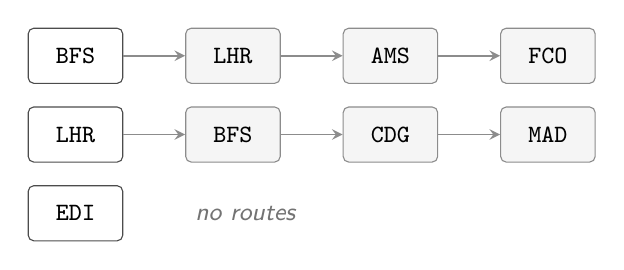
\begin{tikzpicture}
        \DrawAdjacencyList
    \end{tikzpicture}

    \caption{Inside the Graph.}
    \label{fig:adjacency-list}
\end{figure}

%%%%%%%%%%%%%%%%%%%%%%%%%%%%%%%%%%%%%%%%%%%%%%%%%%%%%%%%%%%%%%%%%%%%%%%%%%%%%%%%

\subsection{An Undirected Graph}

Look again at the first two airports in the output.

Belfast lists London Heathrow as one of its routes.

Later in the output, London Heathrow also lists Belfast as one of its routes.

This is exactly what we expect from an \textbf{undirected graph}. A route
between two airports can be travelled in either direction, so both airports
must record the relationship.

\begin{reflectionbox}
Find three examples of routes that appear in two different airport listings.

Why would the graph become inconsistent if only one airport stored the route?
\end{reflectionbox}

%%%%%%%%%%%%%%%%%%%%%%%%%%%%%%%%%%%%%%%%%%%%%%%%%%%%%%%%%%%%%%%%%%%%%%%%%%%%%%%%

\subsection{Looking Ahead}

The demonstration allows us to inspect the airports that are connected
\emph{directly}.

However, many interesting questions cannot be answered simply by examining one
adjacency list.

For example:

\begin{itemize}
    \item Can you travel from Belfast to Lisbon?
    \item Can every airport be reached from Belfast?
    \item Which airports belong to the same connected network?
\end{itemize}

Answering these questions requires us to explore the graph systematically rather
than examining one airport at a time.

In the next part, you will implement your first graph traversal algorithm:
\textbf{Depth-First Search (DFS)}.

%%%%%%%%%%%%%%%%%%%%%%%%%%%%%%%%%%%%%%%%%%%%%%%%%%%%%%%%%%%%%%%%%%%%%%%%%%%%%%%%
\section{Part C -- Exploring the Network with Depth-First Search}
%%%%%%%%%%%%%%%%%%%%%%%%%%%%%%%%%%%%%%%%%%%%%%%%%%%%%%%%%%%%%%%%%%%%%%%%%%%%%%%%

\begin{infobox}[Estimated Effort]
Estimated time: approx. \textbf{45 minutes}
\end{infobox}

\subsection*{Learning Objectives}

By the end of this part of the practical, you should be able to:

\begin{itemize}
    \item explain why graph traversal algorithms are needed to explore connected networks;
    \item describe how Depth-First Search (DFS) systematically visits the vertices of a graph;
    \item explain the purpose of tracking visited vertices when traversing graphs containing cycles;
    \item implement a recursive Depth-First Search algorithm using Test-Driven Development (TDD); and
    \item interpret the results of a graph traversal to identify connected components within a network.
\end{itemize}

In Part B, you displayed the complete flight network using an adjacency list. This allowed you to see which airports are directly connected to one another.

However, an important question still remains unanswered:

\begin{quote}
\textbf{Can we travel from Belfast International Airport (BFS) to Lisbon Airport (LIS)?}
\end{quote}

Simply displaying each airport's immediate neighbours is no longer sufficient. To answer this question, we need a way of systematically exploring the network.

This process is known as \textbf{graph traversal}.

%%%%%%%%%%%%%%%%%%%%%%%%%%%%%%%%%%%%%%%%%%%%%%%%%%%%%%%%%%%%%%%%%%%%%%%%%%%%%%%%
\subsection{Following the Routes}
%%%%%%%%%%%%%%%%%%%%%%%%%%%%%%%%%%%%%%%%%%%%%%%%%%%%%%%%%%%%%%%%%%%%%%%%%%%%%%%%

Imagine arriving at Belfast International Airport (BFS) and deciding to explore every airport that can be reached by following available flight routes.

A simple strategy would be:

\begin{enumerate}
    \item Visit the starting airport.
    \item Choose one available route.
    \item Continue following routes until no unvisited airports remain.
    \item Return to the previous airport whenever you reach a dead end.
\end{enumerate}

This strategy is called \textbf{Depth-First Search (DFS)} because it follows one path as deeply as possible before backtracking to explore alternative routes.

Unlike the linear data structures you have worked with previously, graphs may contain cycles. This means that, without additional care, an algorithm could repeatedly visit the same airports forever.



\begin{figure}[htbp]
    \centering

    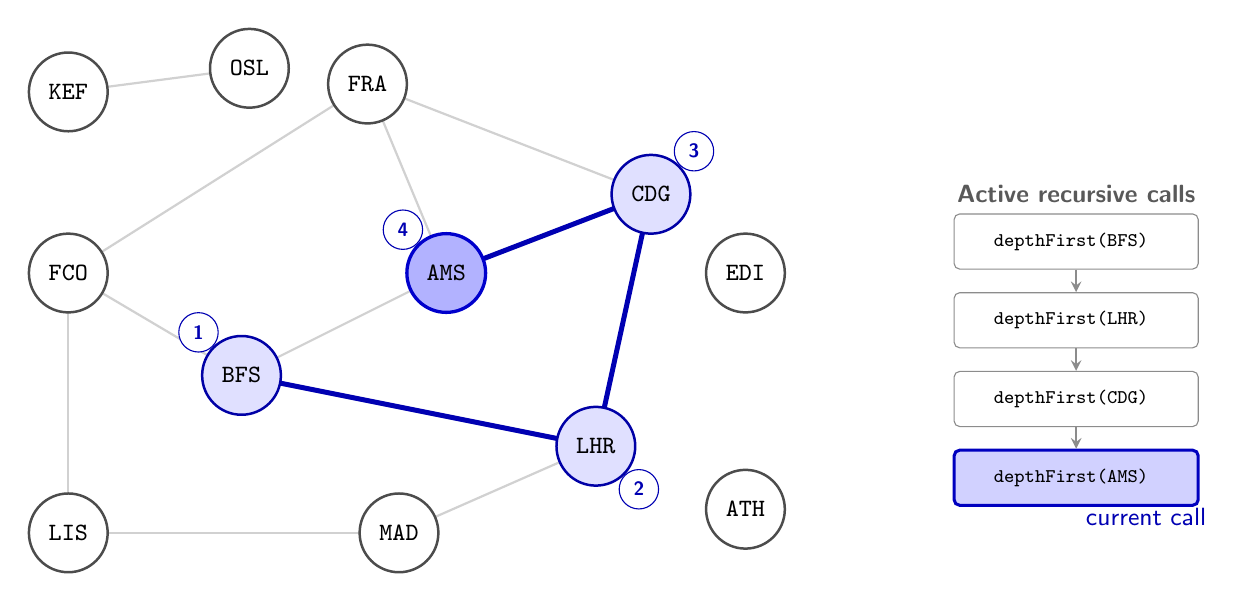
\begin{tikzpicture}
        % Airport network
        \begin{scope}
            \AirportNetworkCoordinates
            \DrawAirportRoutes[route faded]
            \DrawDFSActivePath
            \DrawDFSProgressVertices
        \end{scope}

        % Recursive calls
        \begin{scope}[xshift=13.0cm, yshift=1.2cm]
            \DrawDFSCallStack
        \end{scope}
    \end{tikzpicture}

    \caption{
        Depth-first traversal after reaching \texttt{AMS}.
        The highlighted route corresponds to the active chain of
        recursive function calls. Numbered airports show the order
        in which they were first visited.
    }
    \label{fig:dfs-progress}
\end{figure}

%%%%%%%%%%%%%%%%%%%%%%%%%%%%%%%%%%%%%%%%%%%%%%%%%%%%%%%%%%%%%%%%%%%%%%%%%%%%%%%%
\subsection{Avoiding Infinite Loops}
%%%%%%%%%%%%%%%%%%%%%%%%%%%%%%%%%%%%%%%%%%%%%%%%%%%%%%%%%%%%%%%%%%%%%%%%%%%%%%%%

Consider the following sequence of airports:

\begin{center}
BFS $\rightarrow$ LHR $\rightarrow$ CDG $\rightarrow$ AMS $\rightarrow$ BFS
\end{center}

If our algorithm simply followed every available route, it could continue travelling around this cycle indefinitely.


\begin{figure}[htbp]
    \centering

    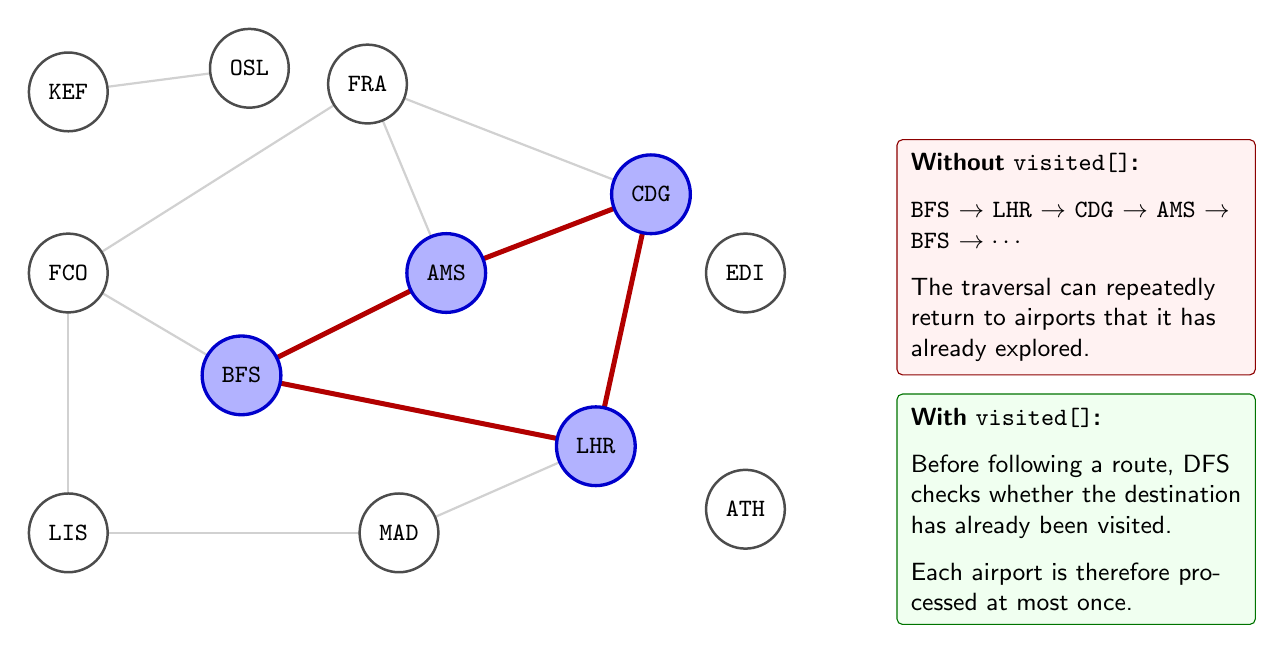
\begin{tikzpicture}
        % Airport network
        \begin{scope}
            \AirportNetworkCoordinates
            \DrawAirportRoutes[route faded]
            \HighlightAirportCycle
            \DrawCycleVertices
        \end{scope}

        % Explanation
        \begin{scope}[xshift=13cm, yshift=1.0cm]
            \DrawVisitedExplanation
        \end{scope}
    \end{tikzpicture}

    \caption{
        Recording visited airports prevents depth-first traversal
        from repeatedly following routes around a cycle.
    }
    \label{fig:dfs-visited-cycle}
\end{figure}


To prevent this, DFS keeps track of every airport that has already been visited.

Whenever the algorithm reaches an airport, it first checks whether it has already been explored.

If it has, that route is ignored and the algorithm continues exploring elsewhere.

This simple idea ensures that every airport is visited at most once.

\begin{importantnote}
The \texttt{visited[]} array is one of the most important components of a graph traversal algorithm. Without it, graphs containing cycles may never terminate.
\end{importantnote}

%%%%%%%%%%%%%%%%%%%%%%%%%%%%%%%%%%%%%%%%%%%%%%%%%%%%%%%%%%%%%%%%%%%%%%%%%%%%%%%%
\subsection{Study the Public Tests}
%%%%%%%%%%%%%%%%%%%%%%%%%%%%%%%%%%%%%%%%%%%%%%%%%%%%%%%%%%%%%%%%%%%%%%%%%%%%%%%%

As in previous sections, your next task is not to begin writing code.

Instead:

\begin{enumerate}
    \item Run the public tests.
    \item Read each failing test carefully.
    \item Examine the TODO comments in \texttt{Graph.cpp}.
    \item Predict how your algorithm should behave before you begin implementing it.
\end{enumerate}

The public tests explore several important situations, including:

\begin{itemize}
    \item traversing the main flight network;
    \item traversing a smaller disconnected component;
    \item traversing an isolated airport;
    \item attempting to start from an airport that does not exist.
\end{itemize}

Together, these tests describe the expected behaviour of your implementation.

%%%%%%%%%%%%%%%%%%%%%%%%%%%%%%%%%%%%%%%%%%%%%%%%%%%%%%%%%%%%%%%%%%%%%%%%%%%%%%%%
\subsection{Implementing Depth-First Search}
%%%%%%%%%%%%%%%%%%%%%%%%%%%%%%%%%%%%%%%%%%%%%%%%%%%%%%%%%%%%%%%%%%%%%%%%%%%%%%%%

Open \texttt{Graph.cpp} and locate the TODO comments for:

\begin{itemize}
    \item \texttt{depthFirstTraversal()}
    \item \texttt{depthFirstTraversalRecursive()}
\end{itemize}

Begin by implementing the public interface (\texttt{depthFirstTraversal()}), then complete the recursive helper function that performs the traversal itself.

Remember to work incrementally:

\begin{enumerate}
    \item Implement a small part of the algorithm.
    \item Compile your project.
    \item Run the public tests.
    \item Fix any failing tests before continuing.
\end{enumerate}

Following this Test-Driven Development (TDD) workflow makes it much easier to identify mistakes while your implementation is still small.

%%%%%%%%%%%%%%%%%%%%%%%%%%%%%%%%%%%%%%%%%%%%%%%%%%%%%%%%%%%%%%%%%%%%%%%%%%%%%%%%
\subsection{Demonstrating Your Traversal}
%%%%%%%%%%%%%%%%%%%%%%%%%%%%%%%%%%%%%%%%%%%%%%%%%%%%%%%%%%%%%%%%%%%%%%%%%%%%%%%%

Once your implementation passes all of the public tests, you can run the demonstration program:

\begin{terminal}
make example03
\end{terminal}

If everything has been implemented correctly, you should see output similar to:

\begin{terminal}
Depth-First Traversal
=====================

Starting from BFS
BFS -> LHR -> CDG -> AMS -> FRA -> FCO -> LIS -> MAD
Visited: 8 airports

Starting from KEF
KEF -> OSL
Visited: 2 airports

Starting from EDI
EDI
Visited: 1 airport
\end{terminal}

Notice that the traversal beginning at Belfast explores every airport in the largest connected component, while the traversal beginning at Keflavík only reaches Oslo. Edinburgh, having no connecting routes, can only reach itself.

\begin{figure}[htbp]
    \centering

    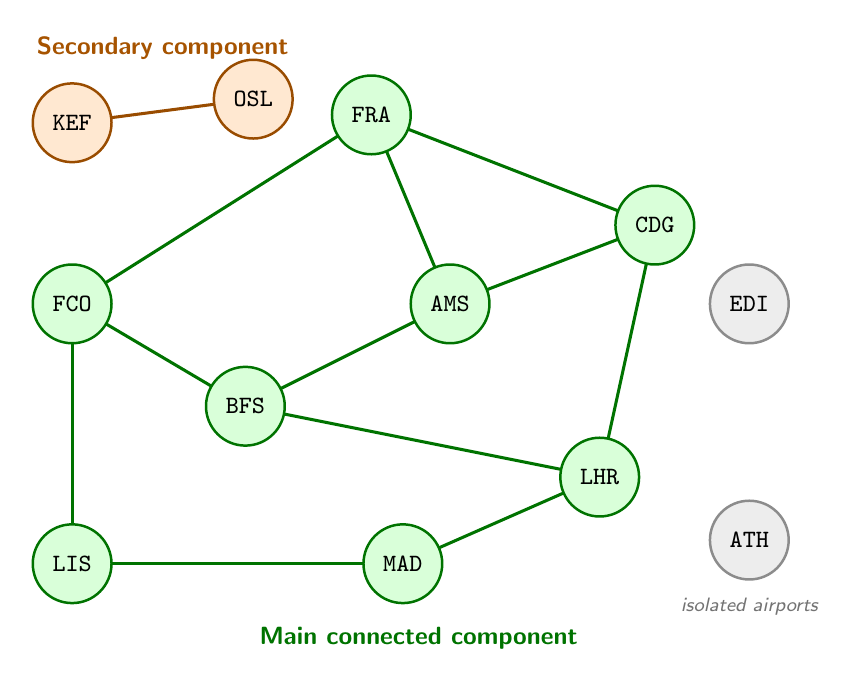
\begin{tikzpicture}
        \AirportNetworkCoordinates
        \DrawConnectedComponentRoutes
        \DrawConnectedComponentVertices
        \DrawConnectedComponentLabels
    \end{tikzpicture}

    \caption{
        The airport network contains four connected components:
        one main network, one two-airport network, and two isolated airports.
    }
    \label{fig:connected-components}
\end{figure}

%%%%%%%%%%%%%%%%%%%%%%%%%%%%%%%%%%%%%%%%%%%%%%%%%%%%%%%%%%%%%%%%%%%%%%%%%%%%%%%%
\subsection{Reflection}
%%%%%%%%%%%%%%%%%%%%%%%%%%%%%%%%%%%%%%%%%%%%%%%%%%%%%%%%%%%%%%%%%%%%%%%%%%%%%%%%

You have now implemented your first graph traversal algorithm.

More importantly, you have discovered an important property of graphs:

\begin{quote}
Starting from any vertex, a traversal can only visit vertices that belong to the same \textbf{connected component}.
\end{quote}

This explains why the traversal starting from Belfast never reaches Oslo, and why the traversal starting from Edinburgh immediately stops.

In the final part of this practical, you'll build upon this idea and explore how graph traversal forms the foundation of many more advanced graph algorithms.

%%%%%%%%%%%%%%%%%%%%%%%%%%%%%%%%%%%%%%%%%%%%%%%%%%%%%%%%%%%%%%%%%%%%%%%%%%%%%%%%
\section{Part D -- Exploring beyond Depth-First Search}
%%%%%%%%%%%%%%%%%%%%%%%%%%%%%%%%%%%%%%%%%%%%%%%%%%%%%%%%%%%%%%%%%%%%%%%%%%%%%%%%
\begin{infobox}[Estimated Effort]
Estimated time: approx. \textbf{20 minutes}
\end{infobox}

Congratulations! You have now implemented a complete graph data structure capable of storing airports and routes, together with a Depth-First Search (DFS) algorithm for exploring the network.

While DFS is a powerful algorithm, it is only one of many techniques used to solve graph problems. In this final part, you'll experiment with your graph and consider how it could be extended to solve increasingly sophisticated problems.

Unlike the previous sections, these activities are intentionally more open-ended. There is often more than one correct solution, and experimentation is encouraged.

%%%%%%%%%%%%%%%%%%%%%%%%%%%%%%%%%%%%%%%%%%%%%%%%%%%%%%%%%%%%%%%%%%%%%%%%%%%%%%%%
\subsection{Experiment with the Flight Network}
%%%%%%%%%%%%%%%%%%%%%%%%%%%%%%%%%%%%%%%%%%%%%%%%%%%%%%%%%%%%%%%%%%%%%%%%%%%%%%%%

Your graph is entirely data-driven. Rather than modifying your algorithms, try changing the flight network itself by editing the dataset.

For example, you could:

\begin{itemize}
    \item Add a new airport to the network.
    \item Add additional routes between existing airports.
    \item Connect the Keflavík (KEF) and Oslo (OSL) component to the main European network.
    \item Introduce a new isolated airport with no routes.
    \item Create additional cycles in the graph.
\end{itemize}

After each change:

\begin{enumerate}
    \item Rebuild the project.
    \item Run:
\begin{terminal}
make example02
\end{terminal}

    \item Then run:

\begin{terminal}
make example03
\end{terminal}

    \item Observe how both the network structure and the DFS traversal change.
\end{enumerate}

\begin{reflectionbox}
Think about the following questions:

\begin{itemize}
    \item Which changes altered the traversal order?
    \item Which changes made previously unreachable airports accessible?
    \item Which airports remained isolated?
    \item Why did the DFS algorithm itself require no modifications?
\end{itemize}
\end{reflectionbox}

%%%%%%%%%%%%%%%%%%%%%%%%%%%%%%%%%%%%%%%%%%%%%%%%%%%%%%%%%%%%%%%%%%%%%%%%%%%%%%%%
\subsection{Challenge: Can One Airport Reach Another?}
%%%%%%%%%%%%%%%%%%%%%%%%%%%%%%%%%%%%%%%%%%%%%%%%%%%%%%%%%%%%%%%%%%%%%%%%%%%%%%%%

Your DFS implementation already discovers every airport that can be reached from a chosen starting point.

Can you reuse this work to answer a simpler question directly?

Implement a member function similar to:

\begin{cppcode}
bool canReach(
    const std::string& source,
    const std::string& destination
) const;
\end{cppcode}

Rather than writing another graph traversal algorithm, reuse your existing \texttt{depthFirstTraversal()} function.

Once implemented, your program should be able to answer questions such as:

\begin{terminal}
Can Belfast reach Lisbon?        Yes
Can Belfast reach Oslo?          No
Can Keflavík reach Oslo?         Yes
Can Edinburgh reach Athens?      No
\end{terminal}

\begin{tipbox}
This challenge demonstrates an important software engineering principle:

Well-designed algorithms become reusable building blocks for solving larger problems.
\end{tipbox}

%%%%%%%%%%%%%%%%%%%%%%%%%%%%%%%%%%%%%%%%%%%%%%%%%%%%%%%%%%%%%%%%%%%%%%%%%%%%%%%%
\subsection{Challenge: Finding the Best Route}
%%%%%%%%%%%%%%%%%%%%%%%%%%%%%%%%%%%%%%%%%%%%%%%%%%%%%%%%%%%%%%%%%%%%%%%%%%%%%%%%

So far, your graph can answer one important question:

\begin{quote}
\textbf{Can I get there?}
\end{quote}

However, real navigation systems need to answer a much more useful question:

\begin{quote}
\textbf{What is the best route?}
\end{quote}

Notice that every flight route in your graph already stores its distance in kilometres.

This means your graph is a \textbf{weighted graph}, where every edge has an associated cost.

\begin{figure}[htbp]
    \centering

    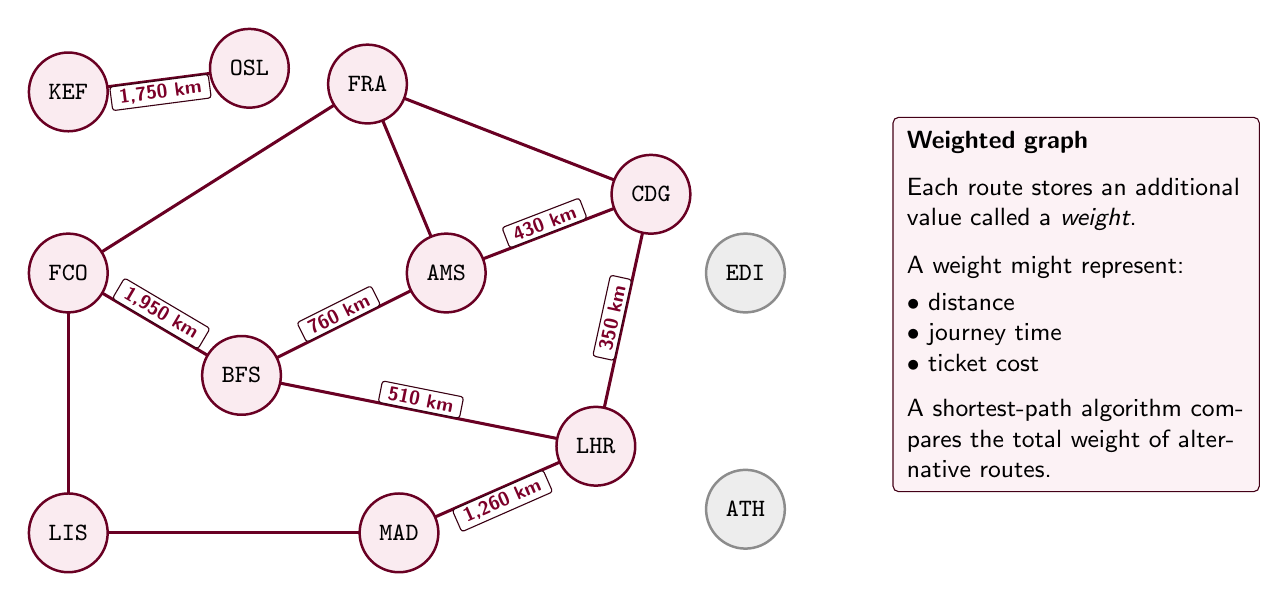
\begin{tikzpicture}
        % Weighted airport network
        \begin{scope}
            \AirportNetworkCoordinates
            \DrawWeightedAirportNetwork
            \DrawWeightedAirportVertices
        \end{scope}

        % Explanation
        \begin{scope}[xshift=13cm, yshift=0.4cm]
            \DrawWeightedGraphExplanation
        \end{scope}
    \end{tikzpicture}

    \caption{
        An illustrative weighted version of the airport network.
        Each route carries a value representing the distance between
        two airports.
    }
    \label{fig:weighted-airport-network}
\end{figure}

Depth-First Search can determine whether a destination is reachable, but it does \emph{not} attempt to minimise the total distance travelled.

Research an algorithm capable of finding the shortest path through a weighted graph.

One of the most famous algorithms for solving this problem is \href{https://www.youtube.com/watch?v=GazC3A4OQTE}{\textbf{Dijkstra's Algorithm}}.  You can also find more information about Dijkstra's Algorithm \href{https://www.youtube.com/watch?v=EFg3u_E6eHU}{here}.
\clearpage
Using your existing graph as a starting point, design and implement a function similar to:

\begin{cppcode}
bool shortestRoute(
    const std::string& source,
    const std::string& destination,
    std::string route[],
    int& numberOfAirports,
    int& totalDistance
) const;
\end{cppcode}

As you research the algorithm, consider the following questions:

\begin{itemize}
    \item How will you keep track of the shortest known distance to every airport?
    \item How will you remember which airport was visited immediately before another?
    \item Once the search finishes, how can you reconstruct the complete route?
    \item How could you display the final journey to the user?
\end{itemize}

\begin{challengebox}
    Modern navigation systems, airline route planners, and mapping applications all build upon graph algorithms like these.
    
    The graph you have developed throughout this practical provides a strong foundation for exploring many more advanced algorithms, including shortest-path algorithms, minimum spanning trees, network optimisation, and route planning.
\end{challengebox}
\begin{tipbox}
Want to learn more about finding the shortest path in a Graph?  

You may enjoy learning about \textbf{A*}, an extension that uses heuristics to guide the search more efficiently.  A* is widely used in robotics, computer games, GPS navigation and Artificial intelligence.  You may want to start learning about\href{https://www.youtube.com/watch?v=ySN5Wnu88nE}{A* here}. 
\end{tipbox}

\end{document}